% Non-Branching Is Not Enough
% Target: arXiv cs.SE (primary), cs.AI / cs.MA (cross-list)
%
% Build:  pdflatex main && bibtex main && pdflatex main && pdflatex main
%
% Every number in this paper is produced by ./scripts/reproduce.sh in the
% accompanying repository. If a figure here is not reproducible from that
% command, it does not belong in the paper.

\documentclass[10pt,conference]{article}

\usepackage[margin=1in]{geometry}
\usepackage{times}
\usepackage{amsmath,amssymb,amsthm}
\usepackage{booktabs}

\newtheorem{definition}{Definition}
\newtheorem{proposition}{Proposition}
\usepackage{listings}
\usepackage{xcolor}
\usepackage{hyperref}
\usepackage{url}
\usepackage{graphicx}
\usepackage{tikz}
\usetikzlibrary{shapes.geometric,positioning,arrows.meta}
% Figures for "Non-Branching Is Not Enough".
% Included from main.tex. Kept separate so a figure can be rebuilt and
% inspected without recompiling the whole paper.
%
% Deliberately monochrome: these are structural diagrams, and the distinctions
% that matter (identical vs differing, admitted vs rejected) are carried by
% shape and label, not by colour. They survive greyscale printing.

% ---------------------------------------------------------------- Figure 1
% The gap, shown on real data: identical control flow, differing output.
\newcommand{\figSequenceVsValue}{%
\begin{figure}[t]
\centering
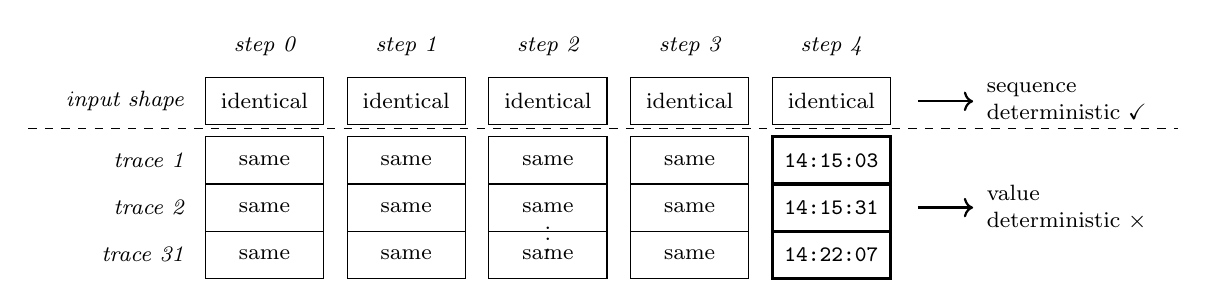
\begin{tikzpicture}[
  font=\footnotesize,
  cell/.style={draw, minimum width=15mm, minimum height=6mm, inner sep=1pt},
  same/.style={cell},
  differs/.style={cell, very thick},
  lbl/.style={font=\footnotesize\itshape},
]

% column headers
\node[lbl] at (0,  0.9) {step 0};
\node[lbl] at (1.8,0.9) {step 1};
\node[lbl] at (3.6,0.9) {step 2};
\node[lbl] at (5.4,0.9) {step 3};
\node[lbl] at (7.2,0.9) {step 4};

% input-shape row
\node[lbl, anchor=east] at (-0.9, 0.2) {input shape};
\foreach \x in {0, 1.8, 3.6, 5.4, 7.2}
  \node[same] at (\x, 0.2) {identical};

% output rows, one per trace
\foreach \y/\name in {-0.55/trace 1, -1.15/trace 2, -1.75/trace 31} {
  \node[lbl, anchor=east] at (-0.9, \y) {\name};
  \foreach \x in {0, 1.8, 3.6, 5.4}
    \node[same] at (\x, \y) {same};
}
\node[differs] at (7.2, -0.55) {\ttfamily 14:15:03};
\node[differs] at (7.2, -1.15) {\ttfamily 14:15:31};
\node[differs] at (7.2, -1.75) {\ttfamily 14:22:07};

% vertical ellipsis between trace 2 and trace 31
\node at (3.6, -1.45) {$\vdots$};

% verdicts
\draw[->, thick] (8.3, 0.2) -- (9.0, 0.2);
\node[anchor=west, align=left] at (9.05, 0.2)
  {sequence\\deterministic \checkmark};
\draw[->, thick] (8.3, -1.15) -- (9.0, -1.15);
\node[anchor=west, align=left] at (9.05, -1.15)
  {value\\deterministic $\times$};

\draw[dashed] (-3.0, -0.15) -- (11.6, -0.15);
\end{tikzpicture}
\caption{The gap, from the corpus. All five steps of the governance workflow
share an identical input shape at every position across 31 traces, so the
published control-flow criterion promotes the workflow. Step~4 appends to an
audit log and returns a different timestamp on every run for byte-identical
input. Promoting it yields an artifact that replays a stale value silently.}
\label{fig:gap}
\end{figure}
}

% ---------------------------------------------------------------- Figure 2
% Two gates and the set each admits. The shaded difference is the finding.
\newcommand{\figTwoGates}{%
\begin{figure}[t]
\centering
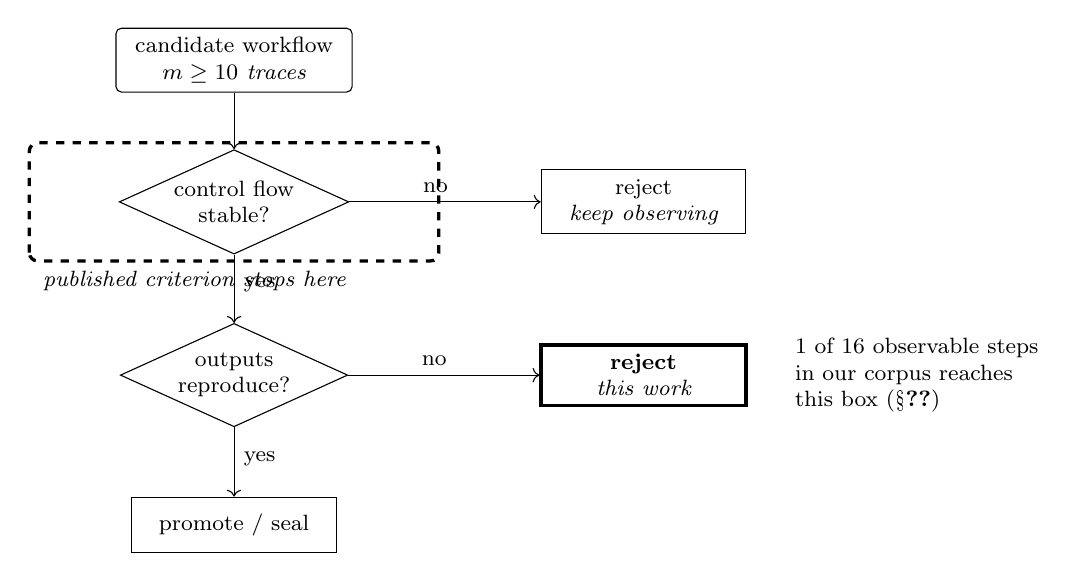
\begin{tikzpicture}[
  font=\footnotesize,
  box/.style={draw, rounded corners=2pt, minimum width=30mm,
              minimum height=8mm, align=center},
  gate/.style={draw, diamond, aspect=2.2, inner sep=1pt, align=center,
               minimum width=26mm},
  % NB: not named "out" - that collides with TikZ's built-in path key.
  result/.style={draw, minimum width=26mm, minimum height=7mm, align=center},
]

\node[box] (cand) at (0,0) {candidate workflow\\\itshape $m \geq 10$ traces};

\node[gate] (cf) at (0,-1.8) {control flow\\stable?};
\node[gate] (pu) at (0,-4.0) {outputs\\reproduce?};

\node[result] (rej1) at (5.2,-1.8) {reject\\\itshape keep observing};
\node[result, very thick] (rej2) at (5.2,-4.0)
  {\textbf{reject}\\\itshape this work};
\node[result] (seal) at (0,-5.9) {promote / seal};

\draw[->] (cand) -- (cf);
\draw[->] (cf) -- node[right, pos=0.45] {yes} (pu);
\draw[->] (cf) -- node[above, pos=0.45] {no} (rej1);
\draw[->] (pu) -- node[right, pos=0.45] {yes} (seal);
\draw[->] (pu) -- node[above, pos=0.45] {no} (rej2);

% what the published criterion does
\draw[dashed, very thick, rounded corners=3pt]
  (-2.6,-2.55) rectangle (2.6,-1.05);
\node[anchor=west, font=\footnotesize\itshape] at (-2.55,-2.8)
  {published criterion stops here};

\node[anchor=west, align=left, font=\footnotesize] at (7.0,-4.0)
  {1 of 16 observable steps\\
   in our corpus reaches\\
   this box (\S\ref{sec:results})};

\end{tikzpicture}
\caption{Two gates. Published promotion criteria test the first. A step that
passes control-flow stability and fails output reproducibility is promoted by
those criteria and rejected here; the bold box is the difference this paper
measures.}
\label{fig:gates}
\end{figure}
}

% ---------------------------------------------------------------- Figure 3
% Oracle vs detector: what each can and cannot see.
\newcommand{\figOracleDetector}{%
\begin{figure}[t]
\centering
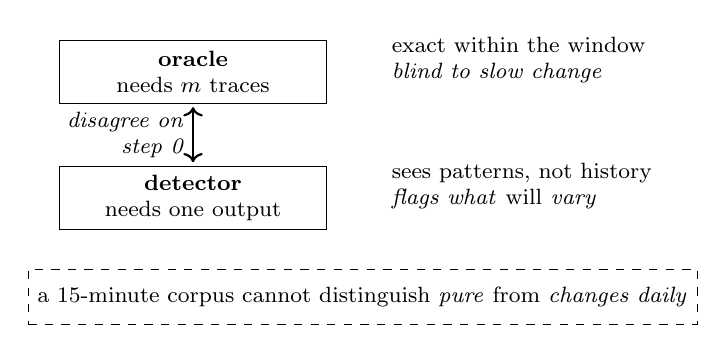
\begin{tikzpicture}[
  font=\footnotesize,
  band/.style={draw, minimum height=8mm, align=center, inner sep=3pt},
]

\node[band, minimum width=34mm] (oracle) at (0,0)
  {\textbf{oracle}\\needs $m$ traces};
\node[band, minimum width=34mm] (det) at (0,-1.6)
  {\textbf{detector}\\needs one output};

\node[align=left, anchor=west, font=\footnotesize] at (2.4, 0.15)
  {exact within the window\\
   \itshape blind to slow change};
\node[align=left, anchor=west, font=\footnotesize] at (2.4, -1.45)
  {sees patterns, not history\\
   \itshape flags what \emph{will} vary};

\draw[<->, thick] (0,-0.45) -- (0,-1.15)
  node[midway, left, font=\footnotesize\itshape, align=right]
  {disagree on\\step 0};

\node[draw, dashed, minimum width=78mm, minimum height=7mm, anchor=north west,
      align=center, font=\footnotesize] at (-2.1,-2.5)
  {a 15-minute corpus cannot distinguish
   \emph{pure} from \emph{changes daily}};

\end{tikzpicture}
\caption{The two purity signals are complementary rather than ranked. The
oracle is exact over observed traces and blind beyond them; the detector
encodes knowledge the observation window cannot supply. Our single false
positive (\S\ref{sec:fp}) is this disagreement, not an error.}
\label{fig:oracle}
\end{figure}
}


\hypersetup{colorlinks=true, linkcolor=black, citecolor=black, urlcolor=blue}

\lstset{
  basicstyle=\ttfamily\footnotesize,
  breaklines=true,
  frame=single,
  framesep=4pt,
  columns=fullflexible,
  keepspaces=true,
  showstringspaces=false,
}

\newcommand{\quench}{\textsc{Quench}}

\title{\textbf{Non-Branching Is Not Enough:\\
Output Purity as a Requirement for Promoting\\
Observed Agent Behaviour to Deterministic Execution}}

\author{
  Shraman Padhalni\\
  \small Independent\\
  \small \texttt{shramanpadhalni@gmail.com}
}

\date{\today}

\begin{document}
\maketitle

\begin{abstract}
A recent class of systems reduces the cost of LLM-agent workflows by observing
execution traces, identifying behaviour that has become repeatable, and
promoting it to deterministic execution without a model in the loop. Published
promotion criteria test \emph{control-flow stability}: that repeated runs
produce the same sequence of actions. We show this is necessary but not
sufficient. A step can be perfectly non-branching and still fail to reproduce,
because its \emph{output} varies for reasons unrelated to its input --- an
embedded timestamp, an identifier, a process attribute. Promoting such a step
yields an artifact that replays a stale value indefinitely, silently.

We report a counterexample drawn from 1{,}399 execution events captured from a
live agent installation across 142 verified sessions. A faithful
reimplementation of a published control-flow-only criterion promotes all five
steps of a cloud governance workflow; one of those steps produces 31 distinct
outputs across 31 traces for byte-identical input. We define output purity
independently of control-flow stability, give an empirical oracle and a cheap
single-trace detector, and measure both. We also report a contrast that was not
anticipated: a corpus built from purpose-written tools exhibited no impurity at
all, while one built from the platform's general-purpose tools did --- which is
the kind these systems actually compile.

Our hypotheses and analysis plan were registered before data collection. The
predicted impurity rate (20\%) was not met (measured 6.2\%, 95\% CI [1.1\%,
28.3\%]); we report this as registered. The existence claim is confirmed. All
artifacts, the corpus, and a single-command reproduction are public.

\textbf{We prove repeatability, not correctness.} Nothing here establishes that
a promoted workflow is right --- only that it reproduces.
\end{abstract}

\section{Introduction}
\label{sec:intro}

Agent workspaces increasingly observe their own use. Repeated work is
synthesised into named, reusable units --- skills, playbooks, recipes --- which
are then re-executed through the model on every invocation. The unit is a
prompt, not a program: the two-hundredth identical run costs what the first did.

A recent line of work closes that gap by treating agent exploration as a
\emph{discovery} mechanism rather than a permanent execution model. Malik's
\emph{Progressive Crystallization}~\cite{malik2026} extracts successful
behaviour from execution traces and promotes it through an execution-type
taxonomy, from agent-orchestrated through hybrid to fully deterministic, on
accumulated evidence. Wang et al.'s LOOP Skill Engine~\cite{loop2026} records a
tool trajectory on first run, extracts a parameterised branch-free template, and
replays it with the LLM bypassed. Both report substantial savings: Malik more
than 70\% cost reduction in production with deterministic execution rising from
zero to roughly 45\% over eight months; LOOP 93.3--99.98\% token reduction.

These systems must decide when observed behaviour has become safe to promote.
The published criteria are properties of control flow. Malik's Type~3 to Type~2
promotion requires ``$\geq 10$ successful runs'' and ``$\geq 90\%$ of runs
produce the same action sequence''~\cite[Table II]{malik2026}. LOOP's templates
are branch-free by construction.

\paragraph{The gap.} Control-flow stability does not imply reproducibility. Two
runs may issue an identical sequence of operations with identical inputs and
still produce different results, because a step's output depends on something
other than its input. We first encountered this in the first trace we ever
captured: a directory listing whose output embedded a modification time.

\begin{lstlisting}
-rw-r--r-- 1 1000 1000 99 Sep 09 14:15 .../quench-test.txt
\end{lstlisting}

\figSequenceVsValue{}

\noindent The step is non-branching. Its input signature is stable. Its output
differs on every execution. A control-flow-only criterion promotes it, and the
resulting artifact replays a frozen timestamp for as long as it is trusted.

\paragraph{Contributions.}
\begin{enumerate}
\itemsep2pt
\item We distinguish \emph{sequence determinism} from \emph{value determinism}
      and argue the latter is a separate, necessary promotion criterion
      (\S\ref{sec:gap}).
\item We reimplement a published control-flow-only criterion and demonstrate,
      on real traces, that it promotes a step that does not reproduce
      (\S\ref{sec:results}).
\item We give an empirical purity oracle and a cheap single-trace detector,
      and measure both, including a disagreement that we argue reflects a limit
      of the oracle rather than an error of the detector (\S\ref{sec:purity},
      \S\ref{sec:fp}).
\item We report a corpus contrast: purpose-written tools exhibited no impurity;
      the platform's general-purpose tools did (\S\ref{sec:contrast}).
\item We implement the criterion in \quench{}, a system that compiles verified
      behaviour into signed, portable artifacts, and demonstrate execution with
      zero model calls and correct refusal on drift (\S\ref{sec:impl}).
\end{enumerate}

\paragraph{Preregistration.} Hypotheses, detector patterns, corpus rules,
exclusion criteria and the analysis plan were committed publicly before data
collection, with a timestamped commit. One deviation was recorded, also before
the corrected analysis ran (\S\ref{sec:method}). Our primary rate prediction was
wrong; we report it as registered rather than adjusting it.

\section{The Gap}
\label{sec:gap}

Let a \emph{workflow} be a finite ordered sequence of operations
$s_1, \dots, s_n$, where each $s_i$ invokes a tool with an input $x_i$ and
yields an output $y_i$.

\paragraph{Structural signature.} Let $\sigma(x)$ denote the recursive shape of
$x$ with leaf values replaced by their types, dictionary keys sorted, and lists
reduced to their element shape. Two inputs share a signature when they differ
only in values.

\begin{definition}[Sequence determinism]
A workflow is \emph{sequence deterministic} over traces
$T_1,\dots,T_m$ if every trace has the same length $n$ and, for each position
$i$, $\sigma(x_i^{(j)})$ is identical across all $j$.
\end{definition}

This is what published criteria test. Malik's $\geq 90\%$ agreement is a relaxed
form of it; LOOP's branch-free templates are a strict form.

\begin{definition}[Value determinism, or purity]
A position $i$ is \emph{pure} over $T_1,\dots,T_m$ if, for every pair of traces
$j, k$ with $x_i^{(j)} = x_i^{(k)}$ (equal as values, not merely as shapes), we
have $y_i^{(j)} = y_i^{(k)}$.
\end{definition}

The quantifier matters and is easy to get wrong. Purity is a claim about traces
sharing identical input \emph{values}. Comparing outputs across traces that
merely share an input \emph{shape} measures the diversity of the corpus, not the
purity of the step --- a mistake we made and corrected under preregistration
(\S\ref{sec:method}).

\begin{proposition}
Sequence determinism does not imply value determinism.
\end{proposition}

\noindent Witness: a step that reads the current time, appends to a log, or
returns a directory listing carrying modification times. Its control flow never
varies; its output always does. We exhibit such a step from real traces in
\S\ref{sec:results}.

\paragraph{Why it matters.} A promoted artifact is executed \emph{in place of}
the agent. If a step is impure, the artifact returns a value that was correct
when observed and is not correct now. Nothing fails; no error is raised; the
audit trail records a successful execution. This is the worst failure shape
available: silent, plausible, and persistent.

\section{Purity: Oracle and Detector}
\label{sec:purity}

\figTwoGates{}

We separate ground truth from what a running system can afford.

\paragraph{Oracle.} Given $m$ traces of one workflow, group positions by
identical serialised input value and check whether serialised outputs agree. The
oracle is exact with respect to the observed traces and requires a corpus.

Positions whose inputs never recur are \emph{unobservable}: with a single
occurrence there is nothing to compare. We exclude them from the denominator
rather than assume purity.

\paragraph{Detector.} A production system sees one output and must judge it.
Detector~v1 is seven regular expressions over the serialised output, frozen at
preregistration: ISO~8601 timestamps, \texttt{ls}-style modification times,
UUIDs, process identifiers, long hexadecimal runs, epoch seconds, and durations
adjacent to \texttt{took}/\texttt{elapsed}/\texttt{duration}.

The detector is deliberately crude. Its purpose is not to match the oracle but
to be affordable, and the interesting question --- how far apart they are, and
in which direction --- is empirical.

\section{Method}
\label{sec:method}

\paragraph{Preregistration.} Before collecting data we committed: three
hypotheses with a point prediction and interval; the seven detector patterns;
corpus size and composition; inclusion and exclusion rules; the baseline
reimplementation; and the analysis plan with its interval estimator. The commit
is public and timestamped.

\paragraph{Deviation.} One deviation was recorded, before the corrected analysis
ran. The registered oracle definition compared outputs across traces sharing an
input \emph{shape}. Because different inputs legitimately produce different
outputs, this classified a pure document-reading step as impure and yielded a
pooled rate of 81.8\% --- an artifact of the definition. We corrected to
comparison within identical input \emph{values} and excluded unobservable
positions. The point prediction, the interval, the falsification thresholds, the
detector patterns and the baseline were left untouched. The flawed figure is
preserved in the deviation record.

\paragraph{Corpus.} 142 verified sessions producing 1{,}399 events across four
workflows with $\geq 10$ traces each, captured from Kiro Crew 0.5.0 / kiro-cli
2.21.2 on Ubuntu 24.04 via a \texttt{postToolUse} hook delivering full
\texttt{tool\_name}, \texttt{tool\_input} and \texttt{tool\_response} grouped by
session. All data is synthetic and committed.

\paragraph{Session verification.} Every session was checked against ground truth
before inclusion: the trace file must have grown, and the artefact the workflow
wrote must match the source document. This is not routine hygiene. During
development a single unknown key in an agent specification caused the runtime to
reject the entire specification and \emph{silently substitute its default
agent}. Four consecutive runs produced confident, plausible, entirely fabricated
results with exit code zero --- including invented lease terms and monetary
values that appear in no document. A system that compiles observed behaviour
must distinguish observation from narration, and narration is convincing. We
return to this in \S\ref{sec:threats}.

\paragraph{Baseline.} We reimplemented the control-flow-only criterion as
published: $\geq 10$ traces, identical step count, $\geq 90\%$ per-position
signature agreement. Written before any purity statistic was computed, per the
preregistration. Two ambiguities and our readings: we interpret ``action'' as
one operation and compare input \emph{shapes} (comparing values would make the
criterion unsatisfiable, since no two runs share a document identifier); and we
could not reproduce the ``zero safety violations'' condition outside its
original environment, so we treat all traces as violation-free --- which makes
our baseline \emph{more} permissive than published.

\section{Results}
\label{sec:results}

\subsection{H3: the existence claim (confirmed)}

The cloud governance workflow --- list a resource directory, read a resource
configuration, read the policy, evaluate compliance, append the finding ---
passes the control-flow-only criterion at every position.

\begin{lstlisting}
workflow: read -> read -> read -> shell -> shell   (31 traces)
baseline: PROMOTE - all positions >= 90% agreement

  [0] pure    read    repeats=1   outputs=1   detector=ls_mtime
  [1] pure    read    repeats=10  outputs=10  detector=-
  [2] pure    read    repeats=1   outputs=1   detector=-
  [3] pure    shell   repeats=10  outputs=10  detector=-
  [4] IMPURE  shell   repeats=10  outputs=31  detector=iso_timestamp
\end{lstlisting}

Step~4 appends the finding to an audit log. Audit entries carry timestamps
because that is what audit entries are; no impurity was contrived. Across 31
traces with byte-identical input it produced 31 distinct outputs.

\textbf{The published criterion promotes this step. Purity rejects it.}

\subsection{H1: the impurity rate (below the registered interval)}

\begin{table}[h]
\centering
\begin{tabular}{lrrr}
\toprule
Corpus & Observable & Impure & Rate \\
\midrule
\texttt{lease-abstraction} & 11 & 0 & 0\% \\
\texttt{cloud-governance-check} & 5 & 1 & 20\% \\
\midrule
Pooled & 16 & 1 & \textbf{6.2\%} \\
\bottomrule
\end{tabular}
\caption{Impurity among observable steps. 95\% Wilson CI [1.1\%, 28.3\%].
Registered prediction: 20\%, interval 8--40\%, falsified below 5\%.}
\end{table}

The measured rate is above the falsification floor and below the predicted
interval. Our prediction was too high. We report it as registered and do not
claim the rate generalises: one impure step over sixteen observable positions
cannot pin down a population parameter, and the interval says so.

\subsection{H2: detector against oracle (below target)}

\begin{table}[h]
\centering
\begin{tabular}{lrrrrrr}
\toprule
& TP & FP & TN & FN & Precision & Recall \\
\midrule
Detector v1 & 1 & 1 & 14 & 0 & 0.50 & 1.00 \\
\bottomrule
\end{tabular}
\caption{Registered targets: precision $\geq 0.80$, recall $\geq 0.70$.}
\end{table}

Recall is perfect. Precision is halved by a single false positive, which we
argue below is not straightforwardly an error.

\section{The False Positive}
\label{sec:fp}

Step~0 is a directory listing. The detector flagged an \texttt{ls}-style
modification time; the oracle scored the step pure.

\figOracleDetector{}

Both are defensible. The pattern is genuinely present, and the listing
\emph{will} return different bytes once any file in that directory changes. But
the directory did not change during a fifteen-minute corpus, so outputs were
byte-identical and the oracle observed purity.

\begin{quote}
\textbf{The oracle is ground truth only within the observation window.} A step
whose output changes daily is indistinguishable from a pure step in a corpus
collected over minutes.
\end{quote}

This is a limitation of every observation-first promotion system, including
those we compare against, and it inverts the usual reading of a precision
failure: the detector encodes knowledge the observation window cannot supply.
We therefore treat the two signals as complementary rather than ranking one
against the other, and recommend that promotion require \emph{both} an observed
purity result and a clean detector pass.

\section{The Corpus Contrast}
\label{sec:contrast}

Our first corpus measured zero impurity across eleven observable steps. The
cause was our own design: its tools were written to be deterministic --- no
clock, no randomness, no network, sorted keys on serialisation --- with a
self-test asserting byte-stable output. A corpus built from tools that cannot be
impure cannot measure impurity.

We record this rather than quietly replacing it, because the second corpus makes
the point sharper than either alone:

\begin{quote}
Purpose-written tools are pure because someone chose to make them so.
General-purpose platform tools are not --- and observation-first systems compile
the second kind.
\end{quote}

This bears directly on the systems under discussion. Malik's system crystallises
workflows built from operational tooling in a production cloud network
environment; LOOP records trajectories over whatever tools an agent has been
given. Neither operates over hand-written pure functions. We expect impurity to
be \emph{more} prevalent in those settings than in ours, not less --- though we
cannot demonstrate that from our data, and do not claim it.

\section{Implementation}
\label{sec:impl}

We implement the criterion in \quench{}, which compiles observed behaviour into
signed, portable artifacts. Three properties are relevant here.

\paragraph{Verification is a gate, not a report.} Branching and purity are
checked independently and both must pass. On our corpus, three workflows seal
and one is refused:

\begin{lstlisting}
CANDIDATE [3]  read -> read -> read -> shell -> shell
  REFUSED - not sealed
    purity: step 4 produced 31 distinct outputs for
            identical input across 31 traces
  (passed: no_branching)
\end{lstlisting}

\paragraph{Artifacts are portable and signed.} A sealed workflow is a file
carrying its steps, their input shapes, inferred data-flow edges, and an
Ed25519 signature over a provenance record: what verified it, against how many
traces, under which strategies, when. To our knowledge no system in this class
produces a transferable, independently verifiable artifact; existing
implementations retain compiled behaviour inside the system that produced it.

\paragraph{Data-flow edges are inferred, not declared.} If a step's input value
is byte-identical to a value reachable inside an earlier step's output, by the
same path, in every trace, that is an edge the agent was already following. On
our corpus this recovers the full dependency structure of a six-step extraction
workflow. Executed without a model:

\begin{lstlisting}
Mill executed 6 steps in 478ms, 0 model calls
  [1] extract_clause  {"clause_type":"term","value":24}
  [2] extract_clause  {"clause_type":"annual_rent","value":521000}
  [3] extract_clause  {"clause_type":"escalation","value":2.5}
  [4] extract_clause  {"clause_type":"renewal","value":"NO"}
\end{lstlisting}

\noindent Values match the source document exactly. The agent path for the same
work takes roughly 27 seconds and six model turns. Execution declines and defers
to the agent on input-shape drift, signature failure, or revocation.

\section{Threats to Validity}
\label{sec:threats}

\paragraph{Sample size.} One impure step. H3 is an existence claim and one
instance suffices; H1 is a rate and this corpus cannot establish one.

\paragraph{Synthetic, self-authored workflows.} Two workflow families, both
written by us. The contrast in \S\ref{sec:contrast} is suggestive, not
controlled.

\paragraph{Observation window.} Fifteen minutes (\S\ref{sec:fp}). Slow-changing
impurity is invisible to our oracle and likely under-counted.

\paragraph{Charitable baseline.} Our reimplementation is more permissive than
published (\S\ref{sec:method}). A stricter reading might reject the workflow for
other reasons --- though not, we note, for the reason purity rejects it.

\paragraph{Narration versus observation.} During development, four runs produced
fabricated results with exit code zero after a schema error silently substituted
a different agent. Any system compiling observed behaviour is exposed to this:
if the agent under observation is not the agent you believe it is, the corpus is
invalid and nothing in the transcript reveals it. We mitigate by verifying every
session against ground truth. We are not aware of published promotion criteria
that address it.

\paragraph{Repeatability, not correctness.} \quench{} compiles what an agent
does. A consistently wrong workflow seals cleanly and becomes cheaper and faster
to be wrong. This is a property of the whole approach, not of our implementation.

\section{Related Work}
\label{sec:related}

\paragraph{Observation-first promotion.} Malik~\cite{malik2026} is the closest
work and the direct subject of our comparison; the framing of agent exploration
as discovery rather than permanent execution is his, as is the evidence-based
promotion ladder with automatic demotion. Our contribution is a criterion his
promotion test does not include. LOOP~\cite{loop2026} reaches similar savings
through one-shot recording and branch-free template replay; being single-shot,
it has no opportunity to observe output variation at all, which makes the purity
question more acute rather than less.

\paragraph{Generation-first compilation.} Compiled AI~\cite{compiledai2026}
constrains an LLM to generate business logic within validated templates,
deployed as static code with no runtime inference. This is a different axis:
the model is asked to write the workflow rather than observed performing it, so
purity of observed steps does not arise.

\paragraph{Specification-first orchestration.} Lobster, duckflux, and
Conductor~\cite{conductor2026} execute deterministic workflows a human authored.
Determinism is asserted by the author; our question does not apply.

\paragraph{Regression testing for agents.} AgentAssay~\cite{agentassay2026}
addresses test efficiency for non-deterministic agent workflows. It is
complementary: our oracle could be seen as a narrow, promotion-time instance of
the same concern.

\section{Conclusion}

Promotion criteria for observed agent behaviour test control-flow stability. We
show this is insufficient, exhibit a counterexample from real traces in which a
published criterion promotes a step that does not reproduce, and give a checker
that rejects it. We also report, from a mistake of our own, that purpose-written
tools may show no impurity at all while general-purpose platform tools do ---
and that the second kind is what these systems compile.

Our registered rate prediction was wrong, and we report it unchanged. The
existence claim stands. Both are reproducible from a single command against a
public corpus.

\section*{Availability}

Source, corpus, preregistration, deviation record and a one-command reproduction
are available at \url{https://github.com/<user>/quench} under Apache-2.0.
Reproduction requires no agent runs, API keys, or credentials.

\begin{thebibliography}{9}
\bibitem{malik2026}
A.~Malik,
\newblock ``Progressive Crystallization: Turning Agent Exploration into
Deterministic, Lower-Cost Workflows in Production,''
\newblock arXiv:2607.07052, 2026.

\bibitem{loop2026}
X.~Wang, K.~Yu, X.~Liang, L.~Wang, and C.~Han,
\newblock ``Good to Go: The LOOP Skill Engine That Hits 99\% Success and Slashes
Token Usage by 99\% via One-Shot Recording and Deterministic Replay,''
\newblock arXiv:2605.14237, 2026.

\bibitem{compiledai2026}
XY.AI Labs,
\newblock ``Compiled AI: Deterministic Code Generation for LLM-Based Workflow
Automation,''
\newblock arXiv:2604.05150, 2026.

\bibitem{conductor2026}
Microsoft,
\newblock ``Conductor: Deterministic orchestration for multi-agent AI
workflows,'' 2026.

\bibitem{agentassay2026}
``AgentAssay: Token-Efficient Regression Testing for Non-Deterministic AI Agent
Workflows,''
\newblock arXiv:2603.02601, 2026.
\end{thebibliography}

\end{document}
